\documentclass[utf8]{beamer}

\usepackage{graphicx}
\usepackage{color}
\usepackage{listings}
\usetheme{Boadilla}

\setbeamertemplate{footline}%{infolines theme}
{
\leavevmode%
\hbox{%
\begin{beamercolorbox}[wd=.333333\paperwidth,ht=2.25ex,dp=1ex,center]{author in head/foot}%
\usebeamerfont{author in head/foot}\insertshortauthor%~~(\insertshortinstitute)
\end{beamercolorbox}%
\begin{beamercolorbox}[wd=.333333\paperwidth,ht=2.25ex,dp=1ex,center]{title in head/foot}%
\usebeamerfont{title in head/foot}\insertshorttitle
\end{beamercolorbox}%
\begin{beamercolorbox}[wd=.333333\paperwidth,ht=2.25ex,dp=1ex,right]{date in head/foot}%
\usebeamerfont{date in head/foot}\insertshortdate{}\hspace*{2em}
\insertframenumber{} / \inserttotalframenumber\hspace*{2ex}
\end{beamercolorbox}}%
\vskip0pt%
}

\newenvironment{program}{\begin{semiverbatim}\small}{\end{semiverbatim}}

\begin{document}


\title[KiCS2]{KiCS2: A New Compiler from Curry to Haskell}

\date{May 04, 2011}

\author[B. Braßel, M. Hanus, \underline{B. Peemöller}, F. Reck]
 {Bernd Braßel \and Michael Hanus \\
   \underline{Björn Peemöller} \and Fabian Reck\\
  \texttt{\{bbr, mh, bjp, fre\}@informatik.uni-kiel.de}}

\institute{Kiel University}

\begin{frame}
\titlepage
\end{frame}

\section{Introduction}

\begin{frame}[fragile]
\frametitle{Curry}
\begin{columns}[t]
\column{.45\textwidth}
\begin{itemize}
\item Lazy functional logic programing language.
\item Haskell-like syntax.
\item Extended by non-determinism, free variables, constraints, unification.
\end{itemize}
\begin{example}<2>
\begin{program}
> xorSelf aBool
False
False
\end{program}
\end{example}
\column{.45\textwidth}
\begin{block}{Running Code Example}
\begin{program}
data Bool = True | False

aBool :: Bool
aBool = True ? False

not True  = False
not False = True

xor True  x = not x
xor False x = x

xorSelf x = xor x x
\end{program}
\end{block}
\end{columns}
\end{frame}


\begin{frame}
\frametitle{KiCS2}
% Compilation strategies
%   - compile to logic language (Pakcs compiles to Prolog)
%   - compile to functional language (KiCS compiles to Haskell)
%   - compile to abstract machine (MCC compiles to C)
\begin{block}{Approach}
\begin{itemize}
\item Compile Curry programs into Haskell
\item Reuse features of Haskell (lazy evaluation, higher-order functions)
\item Benefit from mature Haskell compiler (GHC)
\end{itemize}
\end{block}
\pause
\begin{block}{Goals}
\begin{itemize}
\item Efficient execution of purely functional programs
\item Avoid unsafe operations to enable optimization (in contrast to KiCS)
\item Support for different search strategies (including parallel strategies)
\end{itemize}
\end{block}
\end{frame}

\section{Compilation scheme}

\begin{frame}[fragile]
\frametitle{Representation of Non-Determinism}
\begin{itemize}
  \item No built-in non-determinism in Haskell.
  \item Idea: Explicit representation in data types as constructors.
\end{itemize}
\pause
\begin{block}{Curry}
\begin{program}
data Bool = True | False

aBool :: Bool
aBool = True ? False
\end{program}
\end{block}

\begin{block}{Haskell}
\begin{program}
data Bool = True | False | Choice Bool Bool

aBool :: Bool
aBool = Choice True False
\end{program}
\end{block}
\end{frame}

\begin{frame}[fragile]
\frametitle{Extension of Operations}
\begin{itemize}
  \item Operations have to deal with non-deterministic values.
  \item Non-determinism in arguments is propagated.
%   \item Purely functional Curry programs are Haskell programs (no runtime overhead) (first-order)
\end{itemize}
\pause
\begin{block}{Haskell}
\begin{program}
not True           = False
not False          = True
not (Choice x1 x2) = Choice (not x1) (not x2)

xor True           x = not x
xor False          x = x
xor (Choice x1 x2) x = Choice (xor x1 x) (xor x2 x)

xorSelf x = xor x x
\end{program}
\end{block}
\end{frame}


\begin{frame}[fragile]
\frametitle{Example calls}
\begin{example}
\verb!not aBool!\\
$\leadsto$ \verb!not (Choice True False)!\\
$\leadsto$ \verb!Choice (not True) (not False)!\\
$\leadsto$ \verb!Choice False True!
\end{example}
\pause
\begin{example}
\verb!xorSelf aBool!\\
$\leadsto$ \verb!xor aBool aBool!\\
$\leadsto$ \verb!xor (Choice True False) aBool!\\
$\leadsto$ \verb!Choice (xor True aBool) (xor False aBool)!\\
$\leadsto$ \verb!Choice (not aBool) aBool!\\
$\leadsto$ \verb!Choice (Choice False True) (Choice True False)!
\end{example}
\begin{itemize}
  \item Yields two results \verb!True! and \verb!False!
  \item Only \verb!False! is correct w.r.t. the semantics of Curry.
\end{itemize}
\end{frame}


\begin{frame}[fragile]
\frametitle{Call-Time Choice vs. Run-Time Choice}
\begin{block}{Curry}
\begin{program}
xorSelf x = xor x x
\end{program}
\end{block}
\pause
\begin{block}{Call-Time Choice}
\begin{itemize}
\item Variables denote values
\item Both occurrences of {\tt x} are substituted with the same value in each non-deterministic branch
\end{itemize}
\end{block}
\pause
\begin{block}{Run-Time Choice}
\begin{itemize}
\item Variables denote non-deterministic computations
\item Substitutions of {\tt x} may evaluate to different values in the same non-deterministic branch
\end{itemize}
\end{block}
\pause
\begin{itemize}
\item Call-Time Choice is often more intuitive
\item Curry has Call-Time Choice semantics 
\item Unrestricted propagation violates Call-Time Choice
\end{itemize}
\end{frame}


\begin{frame}[fragile]
\frametitle{Identifying Choices}
\begin{itemize}
\item Choices are annotated with unique identifiers
\item Functions that may introduce non-determinism are supplied with an additional parameter to obtain fresh \verb!ID!s
\item Decisions made for different occurrences of the same Choice have to be consistent
\end{itemize}
\pause
\begin{block}{Choice Identifier}
\begin{program}
type ID = Integer

data Bool = False | True | Choice ID Bool Bool

aBool :: ID -> Bool
aBool i = Choice i True False

xor (Choice i x1 x2) x = Choice i (xor x1 x) (xor x2 x)
\end{program}
\end{block}
\end{frame}

\begin{frame}[fragile]
\frametitle{Example call}
% Mention that (aBool 1) is computed only once due to sharing
% Mention the origin of the initial ID 1
\begin{example}
\verb!xorSelf (aBool 1)!\\
$\leadsto$ \verb!xor (aBool 1) (aBool 1)!\\
$\leadsto$ \verb!xor (Choice 1 True False) (Choice 1 True False)!\\
$\leadsto$ $\dots$\\
$\leadsto$ \verb!Choice 1 (Choice 1 False True) (Choice 1 True False)!
\end{example}
\begin{itemize}
\item The paths to \verb!True! are identified as invalid
\end{itemize}
\end{frame}


% \begin{frame}[fragile]
% \frametitle{Representing Failure}
% \begin{itemize}
%  \item Computing with failure is a common programming pattern in FLP
%  \item Failures do not abort the computation, but are ignored
%  \item Thus, failures have to be represented as well.
% \end{itemize}
% \begin{block}{Curry}
% \begin{program}
% data Bool = True | False
% 
% ensureTrue True = True
% \end{program}
% \end{block}
% \begin{block}{Haskell}
% \begin{program}
% data Bool = True | False | Choice Bool Bool | Fail
% 
% ensureTrue True             = True
% ensureTrue (Choice i x1 x2) = ...
% ensureTrue _                = Fail
% \end{program}
% \end{block}
% \end{frame}


\begin{frame}[fragile]
\frametitle{Higher-Order Functions}
\begin{itemize}
\item Up to now only first-order programs were considered
\item Deterministic higher-order functions can remain unchanged
\end{itemize}
\begin{columns}
\column{.45\textwidth}
\begin{block}{Curry}
\begin{program}
apply :: (a -> b) -> a -> b
apply f x = f x

> apply not True
False
\end{program}
\end{block}
\column{.45\textwidth}
\begin{block}{Haskell (first approach)}
\begin{program}
apply :: (a -> b) -> a -> b
apply f x = f x

> apply not True
False
\end{program}
\end{block}
\end{columns}
\end{frame}


\begin{frame}[fragile]
\frametitle{Higher-Order Functions (cont.)}
\begin{itemize}
\item Non-deterministic functions need an additional parameter
\item An identifier is passed to functional argument when applied
\end{itemize}
\begin{columns}[t]
\column{.45\textwidth}
\begin{block}{Curry}
\begin{program}
apply :: (a -> b) 
      -> a -> b
apply f x = f x

to be = be ? not (to be)

> apply to True
True
False
...
\end{program}
\end{block}
\column{.5\textwidth}
\begin{block}{Haskell}
\begin{program}
apply :: (a -> ID -> b) 
      -> a -> ID -> b
apply f x i = f x i

to be i = 
  Choice il be (not (to be ir))
  where il = leftID  i
        ir = rightID i

> apply to True 1
Choice 2 True (
Choice 6 False (
Choice 14 ...
\end{program}
\end{block}
\end{columns}
\end{frame}

\begin{frame}[fragile]
\frametitle{Higher-Order Optimization}

\begin{itemize}
\item Deterministic functions have to be wrapped
\item This causes an unnecessary overhead
\end{itemize}

\begin{columns}[t]
\column{.45\textwidth}
\begin{block}{Curry}
\begin{program}
> apply not True
False
\end{program}
\end{block}
\column{.45\textwidth}
\begin{block}{Haskell}
\begin{program}
> apply (\\x _ -> not x) True 1
False
\end{program}
\end{block}
\end{columns}
\vspace{3ex}
\begin{itemize}
\item Thus, higher-order functions are translated into
  \begin{itemize}
   \item a deterministic variant
   \item a non-deterministic variant
  \end{itemize}
\item Benchmarks show enormously improved performance
% \item Non-deterministic choice between functions is also possible.
\end{itemize}
\end{frame}


\section{Benchmarks}

\begin{frame}
\frametitle{Benchmark: Reverse of a List}
\begin{itemize}
\item Functional programs run with almost no overhead
\end{itemize}
\begin{center}
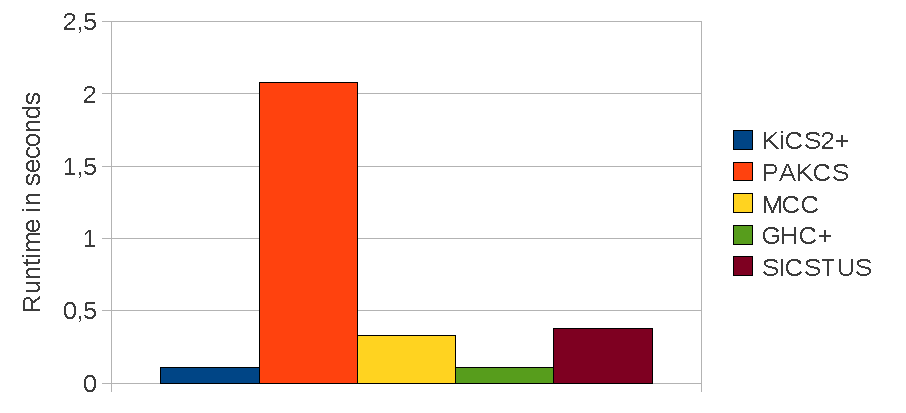
\includegraphics[width=9cm]{reverse}
\end{center}
\end{frame}

\begin{frame}
\frametitle{Benchmark: Reverse using foldr}
\begin{itemize}
\item Higher-order optimization dramatically improves performance
\end{itemize}
\begin{center}
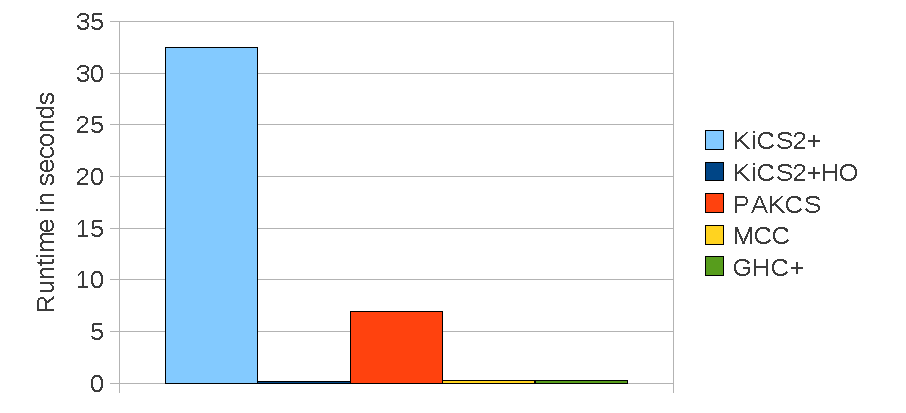
\includegraphics[width=9cm]{reverseho}
\end{center}
\end{frame}

\begin{frame}
\frametitle{Benchmark: Non-Deterministic Permutation Sort}
\begin{itemize}
\item For non-deterministic programs, KiCS2 can compete with existing compilers
\end{itemize}
\begin{center}
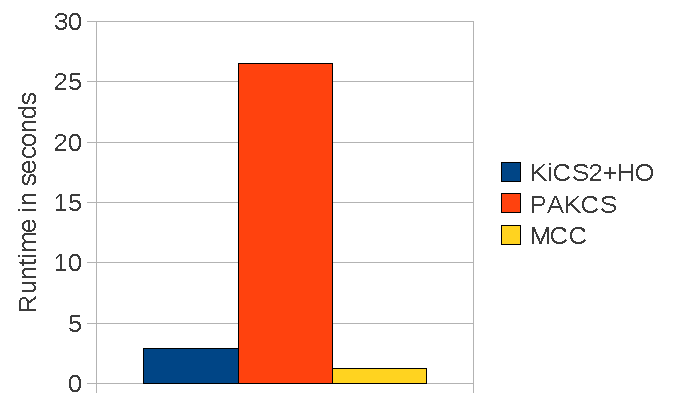
\includegraphics[width=9cm]{permsort}
\end{center}
\end{frame}

\begin{frame}[fragile]
\frametitle{Benchmark: Halve a Peano Number}
\begin{itemize}
\item However, there is still much room for improvements
\end{itemize}
\begin{center}
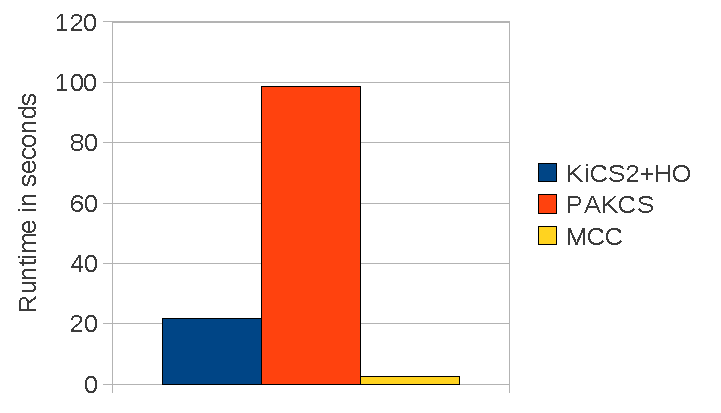
\includegraphics[width=9cm]{half}
\begin{program}
        half y | equal (add x x) y = x where x free
\end{program}
\end{center}
\end{frame}


\section{Conclusion}

\begin{frame}
\frametitle{Status quo}
\begin{itemize}
\item Additional Features (work in progress)
\begin{itemize}
\item Free variables and unification
\item Function Patterns
\item Sharing over non-determinism
\item Different search strategies (depth-first, breadth-first, iterative deepening, parallel)
\item Encapsulated search
\end{itemize}
\item Future work
\begin{itemize}
\item More detailed analysis to decrease overhead of logic features
\item Set Functions
\item First release (coming soon)
\end{itemize}
\end{itemize}
\end{frame}


\begin{frame}
\frametitle{Conclusion}
\begin{itemize}
\item Transformation of a functional logic program into a functional program.
\item Resulting program can be optimized by the Haskell compiler.
\item Our Approach can compete with or outperform existing implementations.
\item A formal description of our approach can be found in our paper (WFLP 2011).
\end{itemize}
\end{frame}

\begin{frame}
\begin{center}
{\huge Thank You!}\\[3ex]
\pause
{\huge Questions?}
\end{center}
\end{frame}

\end{document}